\documentclass{article}
\usepackage{amsmath}
\usepackage{amsfonts}
\usepackage{amssymb}
\usepackage{pgfplots}
\usepackage{tikz}
\usepackage{booktabs}
\usepackage{geometry}

\pgfplotsset{compat=1.18}

\geometry{
    letterpaper,
    total={6.5in, 9in},
    left=1in,
    top=1in
}
 
\begin{document}
Hello World

\begin{equation}
    f(x) = x^2
\end{equation}

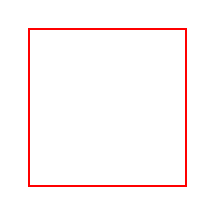
\begin{tikzpicture}
\draw[red, thick] (0,0) rectangle (2,2);
\end{tikzpicture}

\end{document} 